\newpage
\section{Introduction}
\label{sec:intro}

12.5\%

Describe the motivation for making red LEDs [500 Words max + Figures]

LEDs are more energy efficient than traditional incandescent lighting

Narrow wavelengths.

LEDs can be very small for their optical power.

LEDs can be switched on and off very quickly, this is useful for PWM control for dimmable bulbs.

Televisions

LEDs are cost effective for use on a large scale

\hl{The basic function of a Light-Emitting Diode is that two semiconducting layers of types P and N }

Longer Lifetime than incandescent

\cite{einstein}

%
% \subsection{subsection1}
\label{sec:intro:subsection1}
\subsubsection{subsubsection1}
\label{sec:intro:subsubsection1}

Hello World!


%
% This is an example of a citation: \cite{lin_koizumi_yater_koeck_2014, emission_suppression_08}
%
%
%
% \begin{table}[ht]
% \centering
%  \begin{tabular}{| c | c | c | c |}
%  \hline
%  Semiconductor & Electron Mobility ($cm^2.V^{-1}.s^{-1}$) & Hole Mobility ($cm^2.V^{-1}.s^{-1}$) & Band Gap (eV) \\ %[0.5ex]
%  \hline\hline
%  Diamond & 4500 & 3800 & 5.47\\
%  Silicon & 1450 & 480 & 1.12\\
%  GaAs & 8500 & 400 & 1.43\\
%  GaN & 1100 & 200 & 3.45\\
%  \hline
% \end{tabular}
% \caption{Example table}
% \label{tab:example}
% \end{table}
%
%
%
%
% \begin{figure}[!htb]
%   \centering
%   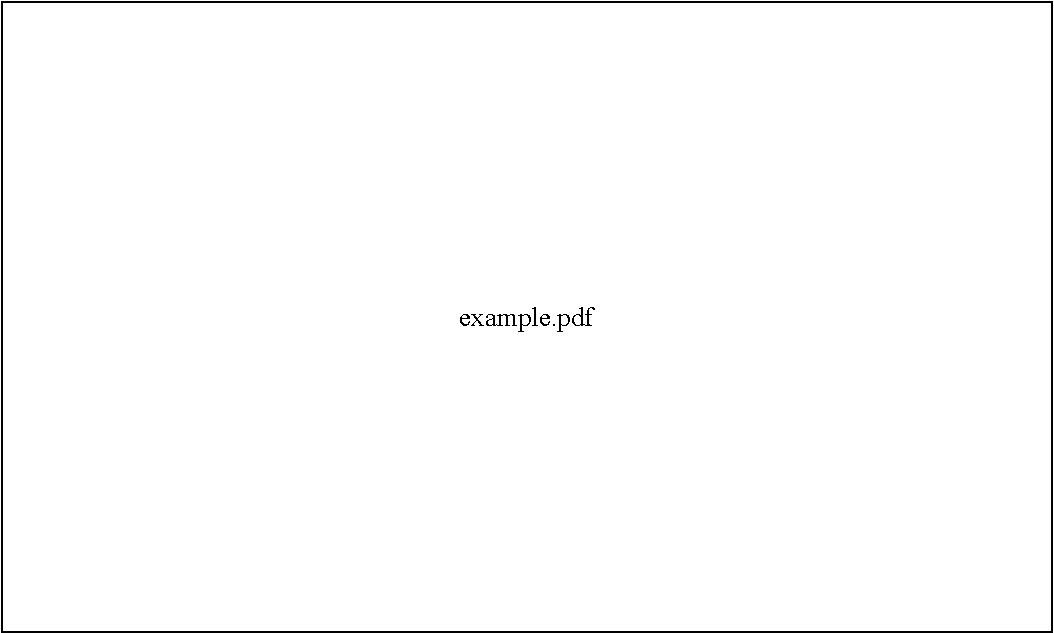
\includegraphics[width=0.67\textwidth]{Figures/example.pdf}
%   \caption{Example Figure}
%   \label{fig:example}
% \end{figure}
%
% Here's an example equation:
%
% \begin{center}
% \begin{equation}
% \%_{err}(V) = \left(\frac{R(V)}{R_{avg}}-1\right)\times100
% \end{equation}
% \end{center}
%
% Here's an example plot with subplots:
%
% \begin{figure*}[!htb]
  \centering
  \begin{subfigure}[t]{0.5\textwidth}
      % \begin{figure}[!htb]
\begin{center}
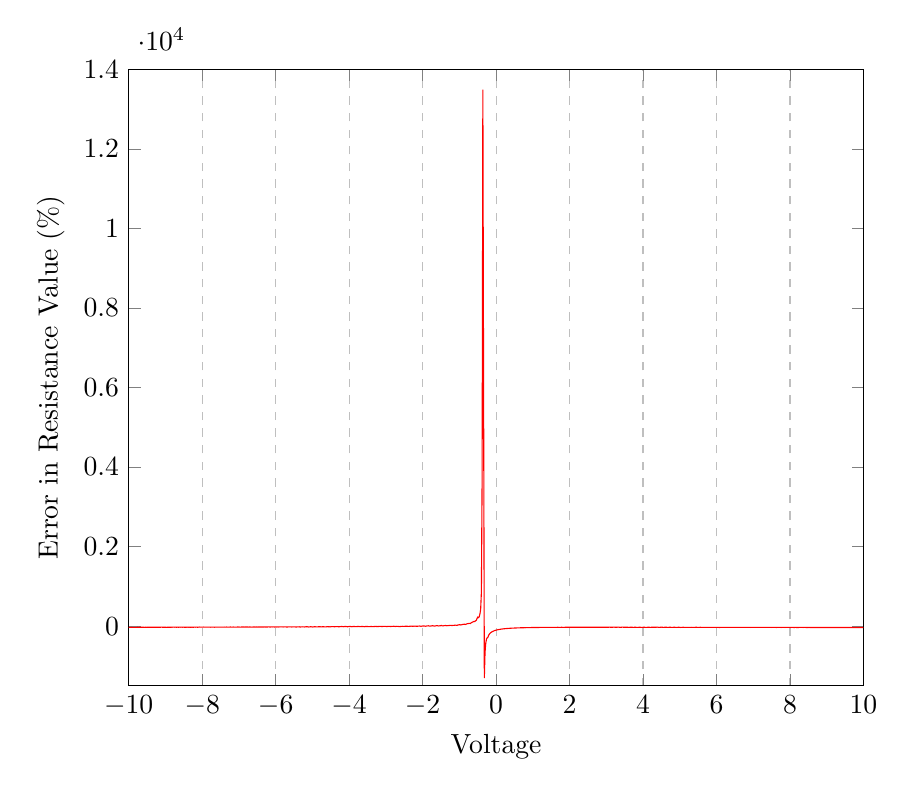
\begin{tikzpicture}

\begin{axis}[
    %title={Temperature dependence of CuSO$_4\cdot$5H$_2$O solubility},
    xlabel={Voltage},
    ylabel={Error in Resistance Value (\%)},
    % height=8cm,
    width=0.9\textwidth,
    xmin=-10, xmax=10,
    ymin=-1500, ymax=14000,
    xtick={-10, -8, -6, -4, -2, 0, 2, 4, 6, 8, 10},
    ytick={-2000, 0, 2000, 4000, 6000, 8000, 10000, 12000, 14000},
    legend pos=south east,
    xmajorgrids=true,
    grid style=dashed,
]

\addplot[color=red]
  coordinates {
  (-10.0,-30.364475134465007)
(-9.98,-28.849073474295984)
(-9.96,-28.423593785412805)
(-9.94,-30.78228828365822)
(-9.92,-28.13613833876788)
(-9.9,-28.85477695538019)
(-9.88,-28.998504678702663)
(-9.86,-28.570798792364048)
(-9.84,-29.847182664035323)
(-9.82,-28.860572428094823)
(-9.8,-29.005459245960196)
(-9.78,-29.150346063825594)
(-9.76,-27.542222126691584)
(-9.74,-29.440119699556366)
(-9.72,-28.43066236196965)
(-9.7,-27.38755644646339)
(-9.68,-29.30465641456027)
(-9.66,-26.461344952595102)
(-9.64,-27.836705581846076)
(-9.62,-28.581575497825117)
(-9.6,-26.293475219249117)
(-9.58,-28.878533603863264)
(-9.56,-28.43557109568967)
(-9.54,-26.75414099912882)
(-9.52,-29.323970762920492)
(-9.5,-26.43246920455763)
(-9.48,-27.214806779008494)
(-9.46,-29.18415298799418)
(-9.44,-25.614599333110622)
(-9.42,-27.675472558888192)
(-9.4,-27.829027818848083)
(-9.38,-26.730106262787256)
(-9.36,-28.136138338767893)
(-9.34,-25.751275673019023)
(-9.32,-25.91026651740229)
(-9.3,-27.981259326566942)
(-9.28,-25.569571850866733)
(-9.26,-26.387239050552058)
(-9.24,-27.190561211646404)
(-9.22,-26.050803067348195)
(-9.2,-27.505753587353578)
(-9.18,-26.371623878335836)
(-9.16,-25.870160718819125)
(-9.14,-27.978542150914286)
(-9.12,-24.14370157981056)
(-9.1,-25.004456293897682)
(-9.08,-27.17367590580495)
(-9.06,-26.679438440229397)
(-9.04,-28.136138338767893)
(-9.02,-28.295129183151147)
(-9.0,-27.165005073075555)
(-8.98,-29.239311653742938)
(-8.96,-28.136138338767868)
(-8.94,-27.650571705921724)
(-8.92,-28.456959149755523)
(-8.9,-25.973568427665995)
(-8.88,-26.81753537250674)
(-8.86,-26.98236074328939)
(-8.84,-25.08531402296087)
(-8.82,-26.63897455415889)
(-8.8,-24.714049688233008)
(-8.78,-24.162895987305532)
(-8.76,-26.457076150421344)
(-8.74,-23.775467121460103)
(-8.72,-24.68114498967019)
(-8.7,-28.30096370955053)
(-8.68,-23.556578527022698)
(-8.66,-25.91178071592022)
(-8.64,-26.082885148446955)
(-8.62,-24.084989274531765)
(-8.6,-26.425094013500463)
(-8.58,-23.689117196364894)
(-8.56,-24.61340002204082)
(-8.54,-26.93840731108069)
(-8.52,-24.22275973345327)
(-8.5,-25.86858930576784)
(-8.48,-26.04301615446015)
(-8.46,-26.217443003152454)
(-8.44,-27.793929473714396)
(-8.42,-24.363285601553198)
(-8.4,-25.290044807629975)
(-8.38,-26.915150397921693)
(-8.36,-23.60352448017542)
(-8.34,-26.550906096240713)
(-8.32,-27.438430943998636)
(-8.3,-24.611975254268625)
(-8.28,-27.07931684374978)
(-8.26,-24.517357919407768)
(-8.24,-27.43159067542247)
(-8.22,-23.797607990798753)
(-8.2,-24.682558074884554)
(-8.18,-26.149951207427304)
(-8.16,-23.003005362965588)
(-8.14,-25.613958046486584)
(-8.12,-26.912004422694803)
(-8.1,-24.754746709413123)
(-8.08,-21.7860988385297)
(-8.06,-23.5450468598824)
(-8.04,-24.214920283800346)
(-8.02,-25.11068470334179)
(-8.0,-25.219706908187177)
(-7.98,-23.250319050236566)
(-7.96,-22.023399833232325)
(-7.94,-22.472953588290345)
(-7.92,-23.82738432053554)
(-7.9,-24.8246150524717)
(-7.88,-25.09428176051468)
(-7.86,-23.086880084792426)
(-7.84,-22.352167113552944)
(-7.82,-23.143408343704163)
(-7.8,-23.757056452990955)
(-7.78,-25.888011171210778)
(-7.76,-25.525698919449624)
(-7.74,-24.752937059261825)
(-7.72,-24.374453104592163)
(-7.7,-23.99014631985065)
(-7.68,-24.436684343063707)
(-7.66,-26.249038005755885)
(-7.64,-24.416312900356086)
(-7.62,-23.433637324022826)
(-7.6,-22.595613856949537)
(-7.58,-23.920660420092265)
(-7.56,-25.454062272377232)
(-7.54,-25.240960689060397)
(-7.52,-23.23632958913843)
(-7.5,-22.64940263214109)
(-7.48,-23.20833068199769)
(-7.46,-23.23820045922228)
(-7.44,-23.879964299606073)
(-7.42,-24.770054525064577)
(-7.4,-23.32863663594035)
(-7.38,-22.18965682806734)
(-7.36,-22.85326402761546)
(-7.34,-21.9703040542243)
(-7.32,-23.717594640339456)
(-7.3,-24.71208522861733)
(-7.28,-23.063395162680912)
(-7.26,-22.63765782020386)
(-7.24,-21.924616082334868)
(-7.22,-22.046712560983185)
(-7.2,-23.63934416161878)
(-7.18,-23.125368485153963)
(-7.16,-21.754067899266726)
(-7.14,-22.350488459261907)
(-7.12,-22.474137116973825)
(-7.1,-22.69190639473515)
(-7.08,-23.558272151213423)
(-7.06,-22.94063436690481)
(-7.04,-21.925681158167563)
(-7.02,-22.33923816781873)
(-7.0,-21.10303769940012)
(-6.98,-22.686536005641145)
(-6.96,-23.66109933422228)
(-6.94,-21.975093878449492)
(-6.92,-20.508644070376235)
(-6.9,-22.13243632812474)
(-6.88,-20.56179816367657)
(-6.86,-22.094486252204113)
(-6.84,-22.321616029894486)
(-6.82,-21.254573179691015)
(-6.8,-20.669763101237272)
(-6.78,-21.514661394466216)
(-6.76,-20.517064000338813)
(-6.74,-22.576338299759513)
(-6.72,-22.209221913099253)
(-6.7,-20.911978789379905)
(-6.68,-22.17078536040361)
(-6.66,-22.80430344132163)
(-6.64,-21.825681285946718)
(-6.62,-22.86985016255566)
(-6.6,-21.159992193462106)
(-6.58,-20.016202684217298)
(-6.56,-23.27035603878863)
(-6.54,-20.9304079299364)
(-6.52,-19.54801201386789)
(-6.5,-22.663062781786625)
(-6.48,-21.655817031496603)
(-6.46,-20.06877645806483)
(-6.44,-20.969387107524796)
(-6.42,-20.123616366843798)
(-6.4,-19.928844945702373)
(-6.38,-22.025265748527055)
(-6.36,-20.760374451207298)
(-6.34,-20.123267368125596)
(-6.32,-21.585012828213568)
(-6.3,-19.153155631113872)
(-6.28,-19.753724887528858)
(-6.26,-20.797927112796998)
(-6.24,-19.693678945901073)
(-6.22,-19.721045342517286)
(-6.2,-18.93086930501471)
(-6.18,-17.877465779139346)
(-6.16,-20.609507203516884)
(-6.14,-21.876042740799374)
(-6.12,-19.034088113633917)
(-6.1,-18.336520839508964)
(-6.08,-19.799508278213796)
(-6.06,-18.38549444020491)
(-6.04,-20.560445747832723)
(-6.02,-20.23959306773281)
(-6.0,-19.314526577957956)
(-5.98,-19.462913655515724)
(-5.96,-19.732268459343437)
(-5.94,-18.660187067888945)
(-5.92,-19.91075658236181)
(-5.9,-19.207929915916633)
(-5.88,-17.59760012323618)
(-5.86,-18.51350051570816)
(-5.84,-18.539411470963596)
(-5.82,-18.692131635231167)
(-5.8,-19.844154300933415)
(-5.78,-19.25094859993748)
(-5.76,-17.608311471198856)
(-5.74,-19.433873840728054)
(-5.72,-19.082423483809507)
(-5.7,-21.588052934719936)
(-5.68,-21.74334082902637)
(-5.66,-18.519740183779287)
(-5.64,-16.807844874928346)
(-5.62,-18.17769397566359)
(-5.6,-16.851730309318224)
(-5.58,-18.09633413609575)
(-5.56,-20.595574158098074)
(-5.54,-17.469777445434097)
(-5.52,-16.521776858164717)
(-5.5,-16.402022179192755)
(-5.48,-16.706014825813863)
(-5.46,-19.857703294459284)
(-5.44,-23.16442463893421)
(-5.42,-17.895841019418622)
(-5.4,-16.938173593610127)
(-5.38,-17.103864550294002)
(-5.36,-15.823798403801536)
(-5.34,-21.23295950924067)
(-5.32,-20.483414301631676)
(-5.3,-16.327226097423065)
(-5.28,-15.90399167302624)
(-5.26,-16.95871873065006)
(-5.24,-17.564221737115528)
(-5.22,-19.9809390205564)
(-5.2,-18.62106257874411)
(-5.18,-14.776830722256785)
(-5.16,-15.569780015492318)
(-5.14,-14.17745145475533)
(-5.12,-17.575499169912977)
(-5.1,-21.147656094603327)
(-5.08,-17.777383504716404)
(-5.06,-15.669958254676597)
(-5.04,-15.69044162648746)
(-5.02,-16.025003366064904)
(-5.0,-19.651317462844233)
(-4.98,-19.54091028036511)
(-4.96,-16.091159642252517)
(-4.94,-14.661664277286857)
(-4.92,-15.816619196842375)
(-4.9,-16.158828061895857)
(-4.88,-18.518669863658754)
(-4.86,-19.003161485717047)
(-4.84,-15.248272309852961)
(-4.82,-13.576892912390514)
(-4.8,-15.784537115743614)
(-4.78,-15.641144710046762)
(-4.76,-16.972820022459977)
(-4.74,-16.017084745009804)
(-4.72,-13.821791910311088)
(-4.7,-12.948414997992009)
(-4.68,-17.080159621655255)
(-4.66,-16.61215255444678)
(-4.64,-16.804311849272203)
(-4.62,-16.327862682738814)
(-4.6,-13.189662909225907)
(-4.58,-13.018898940686285)
(-4.56,-16.06065338749527)
(-4.54,-14.68045712813969)
(-4.52,-17.1365676763344)
(-4.5,-14.53821948320705)
(-4.48,-11.357351254867854)
(-4.46,-12.523792846862658)
(-4.44,-12.53411574126353)
(-4.42,-12.544529586275887)
(-4.4,-14.632561741516914)
(-4.38,-12.759502750499818)
(-4.36,-10.784044179108188)
(-4.34,-11.193291682873753)
(-4.32,-9.541992314533)
(-4.3,-12.410826206548165)
(-4.28,-15.686039498335113)
(-4.26,-12.830281697935986)
(-4.24,-10.170172923459852)
(-4.22,-9.52699993723164)
(-4.2,-7.979201531349123)
(-4.18,-10.597934004776732)
(-4.16,-13.895833954284099)
(-4.14,-10.602047092097067)
(-4.12,-8.842638533166147)
(-4.1,-9.061162712638371)
(-4.08,-8.602071203919259)
(-4.06,-12.539784668884192)
(-4.04,-14.809271974360982)
(-4.02,-9.946158392096926)
(-4.0,-9.033086504769472)
(-3.98,-8.32750980394108)
(-3.96,-8.553697886092792)
(-3.94,-12.609995387267114)
(-3.92,-13.692911240186923)
(-3.9,-9.473817674804508)
(-3.88,-9.470200244941351)
(-3.86,-7.781081777807197)
(-3.84,-10.63561244199116)
(-3.82,-12.684493783108564)
(-3.8,-12.697354759372747)
(-3.78,-8.227906392075202)
(-3.76,-7.967261632754507)
(-3.74,-6.155432048530674)
(-3.72,-10.4110035590538)
(-3.7,-12.76368499128646)
(-3.68,-9.6792995514569)
(-3.66,-6.331291424462404)
(-3.64,-7.632607186834428)
(-3.62,-8.656187073855248)
(-3.6,-10.912568188555227)
(-3.58,-13.317848804848042)
(-3.56,-9.406746631024676)
(-3.54,-7.826786130158803)
(-3.52,-8.081107177493807)
(-3.5,-8.868291371625936)
(-3.48,-10.683486221040084)
(-3.46,-12.447548821174959)
(-3.44,-11.202699671466053)
(-3.42,-9.375218701543576)
(-3.4,-8.829429235750297)
(-3.38,-9.635471571813792)
(-3.36,-10.436730273835348)
(-3.34,-11.233247800105294)
(-3.32,-8.235376647965154)
(-3.3,-7.072592679441225)
(-3.28,-6.462910218713757)
(-3.26,-7.327456876733896)
(-3.24,-7.603606435558696)
(-3.22,-10.724678028870594)
(-3.2,-7.570595934106594)
(-3.18,-6.647434606732794)
(-3.16,-6.316087933377268)
(-3.14,-6.290479395237192)
(-3.12,-9.0035517925957)
(-3.1,-9.586862358027782)
(-3.08,-7.15574919605918)
(-3.06,-6.503649369315356)
(-3.04,-5.507725151321097)
(-3.02,-4.476733179172099)
(-3.0,-7.072592679441225)
(-2.98,-11.065486814588166)
(-2.96,-6.703056790681106)
(-2.94,-7.007150843299992)
(-2.92,-5.646368682195247)
(-2.9,-5.61358749204115)
(-2.88,-8.258900006937731)
(-2.86,-9.537568507427896)
(-2.84,-4.8071981726216295)
(-2.82,-4.766875054194286)
(-2.8,-3.6308368527538604)
(-2.78,-2.8299925008631988)
(-2.76,-6.793111755168879)
(-2.74,-7.119348607652832)
(-2.72,-3.424059427593207)
(-2.7,-5.626251709471431)
(-2.68,-5.218922612154476)
(-2.66,-5.926244085198107)
(-2.64,-11.179496823196256)
(-2.62,-8.777462426149151)
(-2.6,-8.048208504328969)
(-2.58,-3.833629104782754)
(-2.56,-4.181517785023836)
(-2.54,-3.318745434571202)
(-2.52,-6.45819659798299)
(-2.5,-5.242798442468189)
(-2.48,-3.140012543556703)
(-2.46,-0.9052131801395746)
(-2.44,-1.2681179879468818)
(-2.42,-2.077395709357144)
(-2.4,-5.442287287852476)
(-2.38,-4.127807873468359)
(-2.36,-3.1970813239110885)
(-2.34,-2.2317230887888617)
(-2.32,1.1675722415403378)
(-2.3,-0.6689412134411765)
(-2.28,-3.844128763140131)
(-2.26,-1.9249230951784102)
(-2.24,0.10886201564672682)
(-2.22,-0.7849671094929733)
(-2.2,1.3464715735324706)
(-2.18,-2.085488486571241)
(-2.16,-3.4664544849120738)
(-2.14,-1.9204949266347304)
(-2.12,0.23117547487636614)
(-2.1,1.9689928976942328)
(-2.08,3.803355732890834)
(-2.06,-0.5110517324340313)
(-2.04,-2.525081257371342)
(-2.02,0.8090281636728314)
(-2.0,3.8495110711446845)
(-1.98,4.013483983362254)
(-1.96,6.064133174710062)
(-1.94,-0.41722026943550317)
(-1.92,-0.8774321914039818)
(-1.9,2.201599667919929)
(-1.88,5.550046814934673)
(-1.86,8.495765170366653)
(-1.84,10.191254547222584)
(-1.82,3.474864100824737)
(-1.8,1.0585554611076686)
(-1.78,3.829280646910038)
(-1.76,6.107715204503794)
(-1.74,11.645642223699904)
(-1.72,10.36235897974931)
(-1.7,6.790703517565189)
(-1.68,1.2846372406627227)
(-1.66,5.0123330613074835)
(-1.64,8.324203239357232)
(-1.62,13.690874893746141)
(-1.6,14.069621684495438)
(-1.58,6.715132917995059)
(-1.56,5.364308450678679)
(-1.54,8.927506848717993)
(-1.52,10.113981577694364)
(-1.5,16.159259150698468)
(-1.48,15.607081802851663)
(-1.46,6.627274416055773)
(-1.44,7.795792491848186)
(-1.42,12.883499512112383)
(-1.4,14.328870824687456)
(-1.38,16.94826543926924)
(-1.36,14.176228807565039)
(-1.34,11.455526187559073)
(-1.32,15.121720136925255)
(-1.3,15.622549702477407)
(-1.28,12.727626135266057)
(-1.26,19.773102768720218)
(-1.24,21.603696042477914)
(-1.22,20.829535869216052)
(-1.2,13.82871435253239)
(-1.18,18.966549888122742)
(-1.16,18.412044782712012)
(-1.14,21.7669475234908)
(-1.12,25.604751967197203)
(-1.1,25.07950605594198)
(-1.08,21.57420205847538)
(-1.06,20.22678876405626)
(-1.04,28.504842035215617)
(-1.02,32.217061497937884)
(-1.0,37.14477416265672)
(-0.98,36.69756294256108)
(-0.96,30.661566656785656)
(-0.94,35.32057283965984)
(-0.92,41.99903936497758)
(-0.9,43.60007880796826)
(-0.88,46.66094216577983)
(-0.86,51.47774761926376)
(-0.84,43.182267066971015)
(-0.82,46.15170278325975)
(-0.8,57.59618785357921)
(-0.78,62.19274333264193)
(-0.76,63.326958320982094)
(-0.74,67.86381827434269)
(-0.72,70.65296964408682)
(-0.7,67.68234387620826)
(-0.68,82.88707308996199)
(-0.66,93.11949794956513)
(-0.64,104.59462394656826)
(-0.62,110.96398783126853)
(-0.6,119.09713921107357)
(-0.58,115.29462687765819)
(-0.56,136.17231531860324)
(-0.54,142.5405331066584)
(-0.52,190.13360298012964)
(-0.5,227.84608422094945)
(-0.48,214.73224085211146)
(-0.46,235.9489467903128)
(-0.44,304.970531902435)
(-0.42,424.7361247864653)
(-0.4,845.5771271214754)
(-0.38,3735.4308189983435)
(-0.36,13487.70493594725)
(-0.34,5996.2357696654)
(-0.32,-1302.7424545812908)
(-0.3,-645.5252656470049)
(-0.28,-422.4660459157851)
(-0.26,-320.33731169717396)
(-0.24,-290.7890132599083)
(-0.22,-274.8899288215826)
(-0.2,-223.0545576390961)
(-0.18,-196.82256810645043)
(-0.16,-175.25011692275615)
(-0.14,-157.95472714615494)
(-0.12,-146.66484523456631)
(-0.1,-137.58570170566534)
(-0.08,-126.8148737541911)
(-0.06,-118.64979108855505)
(-0.04,-111.47985010562813)
(-0.02,-105.51103233598407)
(0.0,-100.0)
(0.02,-95.05069823269751)
(0.04,-90.83369111463875)
(0.06,-86.7572736496501)
(0.08,-83.24851709528389)
(0.1,-79.94869931327229)
(0.12,-76.96671100601536)
(0.14,-74.01616572166193)
(0.16,-71.65133662278812)
(0.18,-69.14242581340224)
(0.2,-67.09530143716478)
(0.22,-64.89775851360776)
(0.24,-63.272302387785984)
(0.26,-61.52264408583123)
(0.28,-59.82052463030152)
(0.3,-58.088727647026374)
(0.32,-56.77361704587541)
(0.34,-55.282370122952194)
(0.36,-54.12945000346887)
(0.38,-53.11080454795981)
(0.4,-52.026794618670145)
(0.42,-50.61711076944129)
(0.44,-49.326764213233766)
(0.46,-48.21839541953826)
(0.48,-47.608363308943765)
(0.5,-47.03430007279472)
(0.52,-46.49311560160265)
(0.54,-45.312168408870704)
(0.56,-44.59834453429241)
(0.58,-43.244771563841745)
(0.6,-42.72274575353444)
(0.62,-42.760027967672265)
(0.64,-41.98679179718901)
(0.66,-40.71231412948351)
(0.68,-40.11344861563989)
(0.7,-39.537616390790284)
(0.72,-39.5537612195244)
(0.74,-39.569025421236624)
(0.76,-39.044045912347755)
(0.78,-37.43994185740954)
(0.8,-38.577896016040924)
(0.82,-37.57588287901448)
(0.84,-36.590710298912846)
(0.86,-35.621957261812895)
(0.88,-35.731505831418445)
(0.9,-35.835837802471325)
(0.92,-35.9353171237078)
(0.94,-35.54195614355136)
(0.96,-34.170508401924785)
(0.98,-34.30355930223183)
(1.0,-33.45938735071101)
(1.02,-34.0817096272871)
(1.04,-34.209140732674825)
(1.06,-33.41285545375345)
(1.08,-32.627629692594894)
(1.1,-32.31999329849714)
(1.12,-32.02067140153718)
(1.14,-32.18145505479752)
(1.16,-32.33597440987885)
(1.18,-32.05179746774528)
(1.2,-31.340259559332374)
(1.22,-31.504756854138137)
(1.24,-31.241366929068036)
(1.26,-31.815914387686394)
(1.28,-31.963207894691482)
(1.3,-31.306602823822228)
(1.32,-30.65767734442515)
(1.34,-30.82070788358402)
(1.36,-30.97821196378836)
(1.38,-31.130465907985894)
(1.4,-30.90013301804605)
(1.42,-30.295981175580877)
(1.44,-29.31423443157498)
(1.46,-29.865482603342997)
(1.48,-29.65706662789448)
(1.5,-30.18407222030559)
(1.52,-29.978801458286654)
(1.54,-29.777698630521922)
(1.56,-28.86572069065856)
(1.58,-29.73706595003295)
(1.6,-29.545233665458703)
(1.62,-29.357126279614054)
(1.64,-29.51152325094458)
(1.66,-28.651907680834153)
(1.68,-28.136138338767893)
(1.7,-29.300599060130438)
(1.72,-30.08719340649365)
(1.74,-29.274253794941252)
(1.76,-28.783560515896113)
(1.78,-28.29726807343431)
(1.8,-28.45412002753439)
(1.82,-29.224984727574434)
(1.84,-29.66515667198558)
(1.86,-28.59680411864758)
(1.88,-28.440646227162947)
(1.9,-27.679376506175313)
(1.92,-27.226469203815583)
(1.94,-27.38755644646338)
(1.96,-27.54466622632976)
(1.98,-28.569053168052417)
(2.0,-27.847528452578196)
(2.02,-27.126003737103964)
(2.04,-26.698861105543237)
(2.06,-27.71506102434659)
(2.08,-26.727043012077058)
(2.1,-27.72312763956539)
(2.12,-27.58964509419577)
(2.14,-26.346425308890442)
(2.16,-26.78021642063142)
(2.18,-26.102255461563207)
(2.2,-26.25909717597449)
(2.22,-28.2653898885183)
(2.24,-26.829522672200024)
(2.26,-27.494496716792604)
(2.28,-26.59067894820376)
(2.3,-25.94673753546871)
(2.32,-26.35858699025685)
(2.34,-27.7657060621636)
(2.36,-27.14831893448979)
(2.38,-26.277590192356705)
(2.4,-26.669528917110085)
(2.42,-26.558046782017865)
(2.44,-26.93840731108068)
(2.46,-27.068853264591176)
(2.48,-26.71777264808567)
(2.5,-26.36899419955726)
(2.52,-26.50286875555806)
(2.54,-28.697574757996257)
(2.56,-27.68416436605574)
(2.58,-28.024548491467826)
(2.6,-26.78446695955975)
(2.62,-26.451829081082757)
(2.64,-27.47683685563731)
(2.66,-28.45888023245604)
(2.68,-27.920977076309107)
(2.7,-27.815317527780238)
(2.72,-27.280616176134163)
(2.74,-26.307267607868255)
(2.76,-26.64783351146427)
(2.78,-28.85272955191408)
(2.8,-27.723127639565405)
(2.82,-27.829027818848097)
(2.84,-27.3171769523151)
(2.86,-26.8053260857821)
(2.88,-27.935960451132136)
(2.9,-27.232821641908835)
(2.92,-27.540581474172043)
(2.94,-27.643920108211496)
(2.96,-26.951569190505808)
(2.98,-26.255403667192933)
(3.0,-27.361325814118477)
(3.02,-26.877067986212598)
(3.04,-27.755906266486228)
(3.06,-26.893810943028495)
(3.08,-25.2227385416909)
(3.1,-24.940036674589095)
(3.12,-27.013265500311135)
(3.14,-26.35361435500364)
(3.16,-26.839625370652865)
(3.18,-25.99511655352392)
(3.2,-23.7518709164646)
(3.22,-24.67394708685956)
(3.24,-27.41929183840647)
(3.26,-27.513555378831477)
(3.28,-27.606429284753897)
(3.3,-25.704654297598374)
(3.32,-23.725057316083564)
(3.34,-24.992094391088994)
(3.36,-28.476725360859035)
(3.38,-28.726569127064383)
(3.4,-28.13613833876788)
(3.42,-26.326616642262046)
(3.44,-24.630584111390718)
(3.46,-25.997332932183603)
(3.48,-27.970553404064592)
(3.5,-28.21817471052729)
(3.52,-27.47683685563731)
(3.54,-26.218657111148)
(3.56,-25.97356842766598)
(3.58,-27.07692042312614)
(3.6,-29.39140229791605)
(3.62,-29.3078317354184)
(3.64,-28.13613833876788)
(3.66,-26.775686614668825)
(3.68,-25.88032205343772)
(3.7,-27.430052361747048)
(3.72,-28.90064750537673)
(3.74,-29.419421582718453)
(3.76,-28.13613833876788)
(3.78,-27.289775942329385)
(3.8,-26.59067894820376)
(3.82,-29.393016577698905)
(3.84,-30.172765997183358)
(3.86,-29.950882320112125)
(3.88,-28.284006366877424)
(3.9,-27.165005073075555)
(3.92,-26.79149227857851)
(3.94,-29.636278592133568)
(3.96,-30.92696791784485)
(3.98,-31.640016871007692)
(4.0,-28.422448544589518)
(4.02,-27.047291949961338)
(4.04,-26.9793759780237)
(4.06,-31.05688129853441)
(4.08,-31.10795216686394)
(4.1,-30.90013301804605)
(4.12,-27.996325378337474)
(4.14,-27.07931684374978)
(4.16,-26.583088283220626)
(4.18,-28.614319927768474)
(4.2,-29.479388089445113)
(4.22,-28.6098172762713)
(4.24,-27.31326969379194)
(4.26,-26.408641664219047)
(4.28,-25.92068210258346)
(4.3,-26.98142600583693)
(4.32,-27.19233527755096)
(4.34,-28.46578908033317)
(4.36,-26.380066531256563)
(4.38,-24.76966680779239)
(4.4,-25.564738392320773)
(4.42,-28.588518762894346)
(4.44,-29.408065093833923)
(4.46,-28.584486851805877)
(4.48,-26.293475219249107)
(4.5,-25.55539192551921)
(4.52,-26.443692321383793)
(4.54,-28.825931077226485)
(4.56,-29.617867445185052)
(4.58,-28.572811109278838)
(4.6,-26.211213472842022)
(4.62,-25.624766829101166)
(4.64,-26.875368835939252)
(4.66,-30.694206262139556)
(4.68,-31.41866383063493)
(4.7,-28.802666566654512)
(4.72,-26.51702187153041)
(4.74,-25.690509538778304)
(4.76,-29.323970762920492)
(4.78,-30.519971937562794)
(4.8,-31.449416539365238)
(4.82,-29.01971040837319)
(4.84,-27.657843086446864)
(4.86,-27.479574818607123)
(4.88,-29.066414865126877)
(4.9,-30.791485428451782)
(4.92,-32.11017677164708)
(4.94,-29.337683796479563)
(4.96,-27.903569207178126)
(4.98,-27.49553665459158)
(5.0,-30.579731780108077)
(5.02,-32.188611740717064)
(5.04,-30.879033822021018)
(5.06,-29.199544391387366)
(5.08,-28.474056183569907)
(5.1,-27.625257805631176)
(5.12,-30.733627314475076)
(5.14,-31.596250196530917)
(5.16,-31.023525637656668)
(5.18,-29.390211797196063)
(5.2,-28.7934297564011)
(5.22,-29.16741732031125)
(5.24,-29.323078996836283)
(5.26,-30.41165089505138)
(5.28,-30.65767734442515)
(5.3,-29.15207090689542)
(5.32,-28.45888023245604)
(5.34,-29.14456771215298)
(5.36,-30.91996081344974)
(5.38,-30.76153729630574)
(5.4,-30.002732148150525)
(5.42,-28.61031337905461)
(5.44,-28.03030054545236)
(5.46,-28.29373452662146)
(5.48,-31.24756251683798)
(5.5,-30.413514236482975)
(5.52,-29.96318566913819)
(5.54,-28.80440028554615)
(5.56,-27.720139139571177)
(5.58,-30.18796168703426)
(5.6,-32.02067140153719)
(5.62,-31.777888085114103)
(5.64,-30.214845081034937)
(5.66,-29.285560326395377)
(5.68,-28.638682825909367)
(5.7,-30.99325952341254)
(5.72,-31.398316304698316)
(5.74,-31.250239010754612)
(5.76,-30.266872781553744)
(5.78,-29.45429340999972)
(5.8,-29.01730285505002)
(5.82,-30.477447661507494)
(5.84,-31.154043290420674)
(5.86,-31.008809086693933)
(5.88,-30.039816793370054)
(5.9,-29.427965412571655)
(5.92,-29.094323160917646)
(5.94,-30.52224312048848)
(5.96,-31.710998804058764)
(5.98,-31.829648995214455)
(6.0,-30.093519784793653)
(6.02,-29.12509056346374)
(6.04,-28.982702154148875)
(6.06,-31.953905989520848)
(6.08,-32.65532076136077)
(6.1,-32.01464700162596)
(6.12,-29.78818113557781)
(6.14,-29.01478272201331)
(6.16,-29.14830540441904)
(6.18,-30.606458583372753)
(6.2,-31.326149460598153)
(6.22,-30.848821235633707)
(6.24,-29.31423443157497)
(6.26,-29.08767749065053)
(6.28,-29.571621218392995)
(6.3,-31.068463997295638)
(6.32,-31.351329247432446)
(6.34,-30.71519420130602)
(6.36,-29.379765116588953)
(6.38,-28.98211936204138)
(6.4,-30.39819693827397)
(6.42,-31.015850498637832)
(6.44,-31.37555321792188)
(6.46,-31.08067898878274)
(6.48,-29.528174400002392)
(6.5,-28.88016126705104)
(6.52,-30.025033149457382)
(6.54,-30.639070946803713)
(6.56,-31.318920090663948)
(6.58,-30.705713697112046)
(6.6,-29.50334617061059)
(6.62,-29.373698901817612)
(6.64,-29.41182819074242)
(6.66,-29.449687696962577)
(6.68,-31.106401277693664)
(6.7,-30.501173047018582)
(6.72,-29.479388089445123)
(6.74,-29.680251510350686)
(6.76,-29.959673467426594)
(6.78,-30.790201411483842)
(6.8,-31.28877119004804)
(6.82,-30.85333852573321)
(6.84,-29.858902145715238)
(6.86,-29.893900597831013)
(6.88,-30.08719340649365)
(6.9,-31.586555537734316)
(6.92,-32.063125314791485)
(6.94,-31.34151983356952)
(6.96,-29.987055268452465)
(6.98,-30.331978556194407)
(7.0,-30.364475134465007)
(7.02,-31.82644474839873)
(7.04,-31.7797214003406)
(7.06,-30.764347253234348)
(7.08,-30.033534026193166)
(7.1,-30.295981175580867)
(7.12,-30.780479568726648)
(7.14,-31.912424063004607)
(7.16,-31.5035610364188)
(7.18,-30.72200231905927)
(7.2,-30.153914152150207)
(7.22,-30.9295685311374)
(7.24,-31.32334234063878)
(7.26,-31.924369042204447)
(7.28,-31.665502495589116)
(7.3,-30.82724286300178)
(7.32,-30.49108517967506)
(7.34,-30.44821405677165)
(7.36,-30.842308861575784)
(7.38,-31.01517962280268)
(7.4,-31.75146608147873)
(7.42,-31.142839162404133)
(7.44,-30.163645407580088)
(7.46,-31.12738849013469)
(7.48,-31.784050098221282)
(7.5,-32.084304125599694)
(7.52,-31.97177244556074)
(7.54,-30.956483572159765)
(7.56,-30.06040239972776)
(7.58,-31.566825201992522)
(7.6,-31.72933142182949)
(7.62,-32.22739778977862)
(7.64,-32.0495169440825)
(7.66,-31.190352459370253)
(7.68,-30.733627314475076)
(7.7,-29.49136916520294)
(7.72,-31.337993561298028)
(7.74,-31.835013571331295)
(7.76,-32.32238270738335)
(7.78,-31.482739739658594)
(7.8,-30.626470178513543)
(7.82,-28.899873710673685)
(7.84,-29.573415571992523)
(7.86,-32.10938069023024)
(7.88,-31.936631022775362)
(7.9,-31.10139476653716)
(7.92,-30.92696791784485)
(7.94,-28.675117301227125)
(7.96,-30.57811422046023)
(7.98,-31.729331421829478)
(8.0,-32.20390409317725)
(8.02,-32.03441385341019)
(8.04,-31.86492361364315)
(8.06,-31.04491369172252)
(8.08,-31.525943134109024)
(8.1,-32.62762969259491)
(8.12,-32.46127816097169)
(8.14,-31.66216893429562)
(8.16,-31.494262715460962)
(8.18,-32.58642334989923)
(8.2,-33.03594708839734)
(8.22,-32.25677260833394)
(8.24,-32.0919472375513)
(8.26,-31.296817439609125)
(8.28,-30.486825402453054)
(8.3,-30.318919183618387)
(8.32,-32.05598533847144)
(8.34,-31.89265838015046)
(8.36,-32.34438249010131)
(8.38,-31.56600446350849)
(8.4,-32.02067140153718)
(8.42,-31.85881585725513)
(8.44,-32.9058636702656)
(8.46,-32.746872825882335)
(8.48,-32.587881981499066)
(8.5,-32.428891137115826)
(8.52,-31.665167259631954)
(8.54,-32.70642778652169)
(8.56,-32.548831598668095)
(8.58,-32.97913771159004)
(8.6,-32.82291192536999)
(8.62,-32.07604303510736)
(8.64,-33.092266729197675)
(8.66,-32.35423456670977)
(8.68,-32.19800878048971)
(8.7,-33.20346191744451)
(8.72,-31.885557208049566)
(8.74,-32.89635139752471)
(8.76,-33.31277244148375)
(8.78,-32.00811364379117)
(8.8,-33.008264553088694)
(8.82,-32.282130357685126)
(8.84,-32.12857509772523)
(8.86,-33.11829681528188)
(8.88,-32.39924877629859)
(8.9,-32.24699483210107)
(8.92,-33.226495206438486)
(8.94,-31.94248694370603)
(8.96,-32.92706244951668)
(8.98,-33.332905194435504)
(9.0,-32.627629692594894)
(9.02,-33.03594708839736)
(9.04,-32.88746803537828)
(9.06,-32.17848055721218)
(9.08,-33.14304673319799)
(9.1,-32.44203087632106)
(9.12,-32.84852270999623)
(9.14,-33.24840492035959)
(9.16,-32.55399868679445)
(9.18,-32.9562754014115)
(9.2,-32.81021064193745)
(9.22,-32.6641458824634)
(9.24,-33.59779182502153)
(9.26,-32.3720163635153)
(9.28,-32.77251651046028)
(9.3,-33.16660865505412)
(9.32,-31.933822085093155)
(9.34,-33.4118583416758)
(9.36,-33.26927131457018)
(9.38,-32.59169776176426)
(9.4,-33.51178153389941)
(9.42,-32.84151023325331)
(9.44,-33.228852944681975)
(9.46,-33.61014342624454)
(9.48,-32.413749151936464)
(9.5,-33.84625137774175)
(9.52,-33.706980328010694)
(9.54,-32.521531471638355)
(9.56,-33.94052716525201)
(9.58,-33.28916717881747)
(9.6,-33.1498961290864)
(9.62,-34.033363627762135)
(9.64,-32.87135402962426)
(9.66,-33.24952849543248)
(9.68,-33.62192930527416)
(9.7,-32.453540880431056)
(9.72,-33.852581880002255)
(9.74,-33.21049498278617)
(9.76,-32.558529825612936)
(9.78,-34.437633671002786)
(9.8,-32.79906066029821)
(9.82,-33.17205288699817)
(9.84,-34.03541056468992)
(9.86,-32.89984128979654)
(9.88,-33.767261827148)
(9.9,-33.633187458377044)
(9.92,-32.49152389399408)
(9.94,-33.858631026606744)
(9.96,-33.72554980130816)
(9.98,-33.09688998329323)
(10.0,-34.43078315581012)

};


\end{axis}
\end{tikzpicture}

% \caption{Percentage Error vs Voltage of 14um gap at $300\degree C$}
\caption{Full}
\label{fig:err_res_sub1}
\end{center}
% \end{figure}

  \end{subfigure}%
  ~
  \begin{subfigure}[t]{0.5\textwidth}
      % \begin{figure}[!htb]
\begin{center}
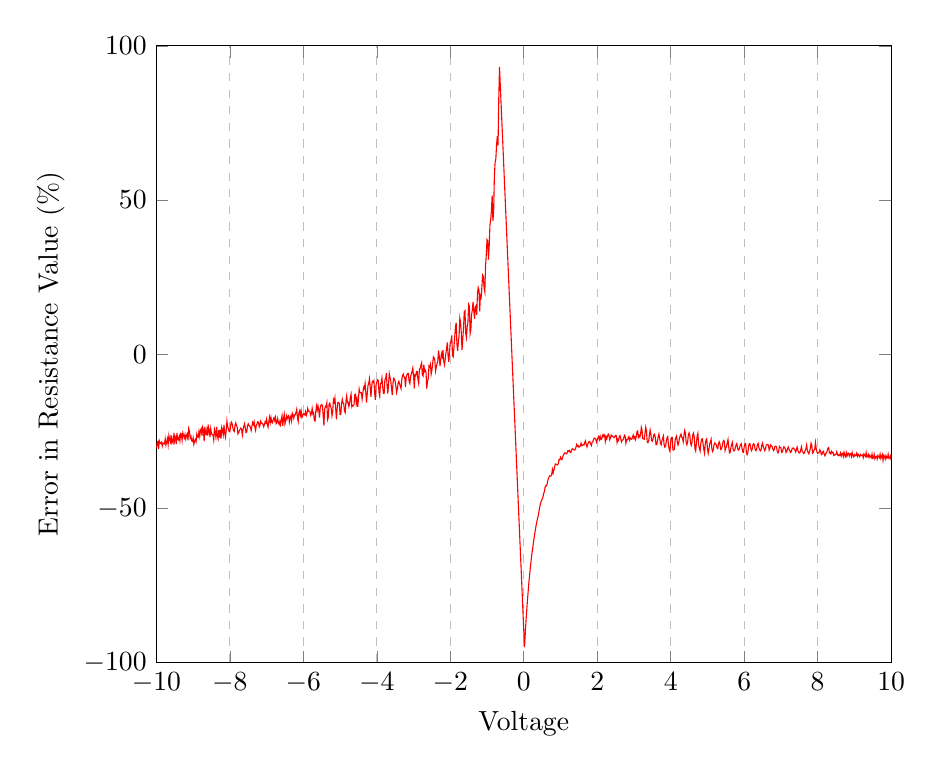
\begin{tikzpicture}

\begin{axis}[
    %title={Temperature dependence of CuSO$_4\cdot$5H$_2$O solubility},
    xlabel={Voltage},
    ylabel={Error in Resistance Value (\%)},
    % height=8cm,
    width=0.9\textwidth,
    xmin=-10, xmax=10,
    ymin=-100, ymax=100,
    xtick={-10, -8, -6, -4, -2, 0, 2, 4, 6, 8, 10},
    ytick={-100, -50, 0, 50, 100},
    legend pos=south east,
    xmajorgrids=true,
    grid style=dashed,
]

\addplot[color=red]
  coordinates {
  (-10.0,-30.364475134465007)
(-9.98,-28.849073474295984)
(-9.96,-28.423593785412805)
(-9.94,-30.78228828365822)
(-9.92,-28.13613833876788)
(-9.9,-28.85477695538019)
(-9.88,-28.998504678702663)
(-9.86,-28.570798792364048)
(-9.84,-29.847182664035323)
(-9.82,-28.860572428094823)
(-9.8,-29.005459245960196)
(-9.78,-29.150346063825594)
(-9.76,-27.542222126691584)
(-9.74,-29.440119699556366)
(-9.72,-28.43066236196965)
(-9.7,-27.38755644646339)
(-9.68,-29.30465641456027)
(-9.66,-26.461344952595102)
(-9.64,-27.836705581846076)
(-9.62,-28.581575497825117)
(-9.6,-26.293475219249117)
(-9.58,-28.878533603863264)
(-9.56,-28.43557109568967)
(-9.54,-26.75414099912882)
(-9.52,-29.323970762920492)
(-9.5,-26.43246920455763)
(-9.48,-27.214806779008494)
(-9.46,-29.18415298799418)
(-9.44,-25.614599333110622)
(-9.42,-27.675472558888192)
(-9.4,-27.829027818848083)
(-9.38,-26.730106262787256)
(-9.36,-28.136138338767893)
(-9.34,-25.751275673019023)
(-9.32,-25.91026651740229)
(-9.3,-27.981259326566942)
(-9.28,-25.569571850866733)
(-9.26,-26.387239050552058)
(-9.24,-27.190561211646404)
(-9.22,-26.050803067348195)
(-9.2,-27.505753587353578)
(-9.18,-26.371623878335836)
(-9.16,-25.870160718819125)
(-9.14,-27.978542150914286)
(-9.12,-24.14370157981056)
(-9.1,-25.004456293897682)
(-9.08,-27.17367590580495)
(-9.06,-26.679438440229397)
(-9.04,-28.136138338767893)
(-9.02,-28.295129183151147)
(-9.0,-27.165005073075555)
(-8.98,-29.239311653742938)
(-8.96,-28.136138338767868)
(-8.94,-27.650571705921724)
(-8.92,-28.456959149755523)
(-8.9,-25.973568427665995)
(-8.88,-26.81753537250674)
(-8.86,-26.98236074328939)
(-8.84,-25.08531402296087)
(-8.82,-26.63897455415889)
(-8.8,-24.714049688233008)
(-8.78,-24.162895987305532)
(-8.76,-26.457076150421344)
(-8.74,-23.775467121460103)
(-8.72,-24.68114498967019)
(-8.7,-28.30096370955053)
(-8.68,-23.556578527022698)
(-8.66,-25.91178071592022)
(-8.64,-26.082885148446955)
(-8.62,-24.084989274531765)
(-8.6,-26.425094013500463)
(-8.58,-23.689117196364894)
(-8.56,-24.61340002204082)
(-8.54,-26.93840731108069)
(-8.52,-24.22275973345327)
(-8.5,-25.86858930576784)
(-8.48,-26.04301615446015)
(-8.46,-26.217443003152454)
(-8.44,-27.793929473714396)
(-8.42,-24.363285601553198)
(-8.4,-25.290044807629975)
(-8.38,-26.915150397921693)
(-8.36,-23.60352448017542)
(-8.34,-26.550906096240713)
(-8.32,-27.438430943998636)
(-8.3,-24.611975254268625)
(-8.28,-27.07931684374978)
(-8.26,-24.517357919407768)
(-8.24,-27.43159067542247)
(-8.22,-23.797607990798753)
(-8.2,-24.682558074884554)
(-8.18,-26.149951207427304)
(-8.16,-23.003005362965588)
(-8.14,-25.613958046486584)
(-8.12,-26.912004422694803)
(-8.1,-24.754746709413123)
(-8.08,-21.7860988385297)
(-8.06,-23.5450468598824)
(-8.04,-24.214920283800346)
(-8.02,-25.11068470334179)
(-8.0,-25.219706908187177)
(-7.98,-23.250319050236566)
(-7.96,-22.023399833232325)
(-7.94,-22.472953588290345)
(-7.92,-23.82738432053554)
(-7.9,-24.8246150524717)
(-7.88,-25.09428176051468)
(-7.86,-23.086880084792426)
(-7.84,-22.352167113552944)
(-7.82,-23.143408343704163)
(-7.8,-23.757056452990955)
(-7.78,-25.888011171210778)
(-7.76,-25.525698919449624)
(-7.74,-24.752937059261825)
(-7.72,-24.374453104592163)
(-7.7,-23.99014631985065)
(-7.68,-24.436684343063707)
(-7.66,-26.249038005755885)
(-7.64,-24.416312900356086)
(-7.62,-23.433637324022826)
(-7.6,-22.595613856949537)
(-7.58,-23.920660420092265)
(-7.56,-25.454062272377232)
(-7.54,-25.240960689060397)
(-7.52,-23.23632958913843)
(-7.5,-22.64940263214109)
(-7.48,-23.20833068199769)
(-7.46,-23.23820045922228)
(-7.44,-23.879964299606073)
(-7.42,-24.770054525064577)
(-7.4,-23.32863663594035)
(-7.38,-22.18965682806734)
(-7.36,-22.85326402761546)
(-7.34,-21.9703040542243)
(-7.32,-23.717594640339456)
(-7.3,-24.71208522861733)
(-7.28,-23.063395162680912)
(-7.26,-22.63765782020386)
(-7.24,-21.924616082334868)
(-7.22,-22.046712560983185)
(-7.2,-23.63934416161878)
(-7.18,-23.125368485153963)
(-7.16,-21.754067899266726)
(-7.14,-22.350488459261907)
(-7.12,-22.474137116973825)
(-7.1,-22.69190639473515)
(-7.08,-23.558272151213423)
(-7.06,-22.94063436690481)
(-7.04,-21.925681158167563)
(-7.02,-22.33923816781873)
(-7.0,-21.10303769940012)
(-6.98,-22.686536005641145)
(-6.96,-23.66109933422228)
(-6.94,-21.975093878449492)
(-6.92,-20.508644070376235)
(-6.9,-22.13243632812474)
(-6.88,-20.56179816367657)
(-6.86,-22.094486252204113)
(-6.84,-22.321616029894486)
(-6.82,-21.254573179691015)
(-6.8,-20.669763101237272)
(-6.78,-21.514661394466216)
(-6.76,-20.517064000338813)
(-6.74,-22.576338299759513)
(-6.72,-22.209221913099253)
(-6.7,-20.911978789379905)
(-6.68,-22.17078536040361)
(-6.66,-22.80430344132163)
(-6.64,-21.825681285946718)
(-6.62,-22.86985016255566)
(-6.6,-21.159992193462106)
(-6.58,-20.016202684217298)
(-6.56,-23.27035603878863)
(-6.54,-20.9304079299364)
(-6.52,-19.54801201386789)
(-6.5,-22.663062781786625)
(-6.48,-21.655817031496603)
(-6.46,-20.06877645806483)
(-6.44,-20.969387107524796)
(-6.42,-20.123616366843798)
(-6.4,-19.928844945702373)
(-6.38,-22.025265748527055)
(-6.36,-20.760374451207298)
(-6.34,-20.123267368125596)
(-6.32,-21.585012828213568)
(-6.3,-19.153155631113872)
(-6.28,-19.753724887528858)
(-6.26,-20.797927112796998)
(-6.24,-19.693678945901073)
(-6.22,-19.721045342517286)
(-6.2,-18.93086930501471)
(-6.18,-17.877465779139346)
(-6.16,-20.609507203516884)
(-6.14,-21.876042740799374)
(-6.12,-19.034088113633917)
(-6.1,-18.336520839508964)
(-6.08,-19.799508278213796)
(-6.06,-18.38549444020491)
(-6.04,-20.560445747832723)
(-6.02,-20.23959306773281)
(-6.0,-19.314526577957956)
(-5.98,-19.462913655515724)
(-5.96,-19.732268459343437)
(-5.94,-18.660187067888945)
(-5.92,-19.91075658236181)
(-5.9,-19.207929915916633)
(-5.88,-17.59760012323618)
(-5.86,-18.51350051570816)
(-5.84,-18.539411470963596)
(-5.82,-18.692131635231167)
(-5.8,-19.844154300933415)
(-5.78,-19.25094859993748)
(-5.76,-17.608311471198856)
(-5.74,-19.433873840728054)
(-5.72,-19.082423483809507)
(-5.7,-21.588052934719936)
(-5.68,-21.74334082902637)
(-5.66,-18.519740183779287)
(-5.64,-16.807844874928346)
(-5.62,-18.17769397566359)
(-5.6,-16.851730309318224)
(-5.58,-18.09633413609575)
(-5.56,-20.595574158098074)
(-5.54,-17.469777445434097)
(-5.52,-16.521776858164717)
(-5.5,-16.402022179192755)
(-5.48,-16.706014825813863)
(-5.46,-19.857703294459284)
(-5.44,-23.16442463893421)
(-5.42,-17.895841019418622)
(-5.4,-16.938173593610127)
(-5.38,-17.103864550294002)
(-5.36,-15.823798403801536)
(-5.34,-21.23295950924067)
(-5.32,-20.483414301631676)
(-5.3,-16.327226097423065)
(-5.28,-15.90399167302624)
(-5.26,-16.95871873065006)
(-5.24,-17.564221737115528)
(-5.22,-19.9809390205564)
(-5.2,-18.62106257874411)
(-5.18,-14.776830722256785)
(-5.16,-15.569780015492318)
(-5.14,-14.17745145475533)
(-5.12,-17.575499169912977)
(-5.1,-21.147656094603327)
(-5.08,-17.777383504716404)
(-5.06,-15.669958254676597)
(-5.04,-15.69044162648746)
(-5.02,-16.025003366064904)
(-5.0,-19.651317462844233)
(-4.98,-19.54091028036511)
(-4.96,-16.091159642252517)
(-4.94,-14.661664277286857)
(-4.92,-15.816619196842375)
(-4.9,-16.158828061895857)
(-4.88,-18.518669863658754)
(-4.86,-19.003161485717047)
(-4.84,-15.248272309852961)
(-4.82,-13.576892912390514)
(-4.8,-15.784537115743614)
(-4.78,-15.641144710046762)
(-4.76,-16.972820022459977)
(-4.74,-16.017084745009804)
(-4.72,-13.821791910311088)
(-4.7,-12.948414997992009)
(-4.68,-17.080159621655255)
(-4.66,-16.61215255444678)
(-4.64,-16.804311849272203)
(-4.62,-16.327862682738814)
(-4.6,-13.189662909225907)
(-4.58,-13.018898940686285)
(-4.56,-16.06065338749527)
(-4.54,-14.68045712813969)
(-4.52,-17.1365676763344)
(-4.5,-14.53821948320705)
(-4.48,-11.357351254867854)
(-4.46,-12.523792846862658)
(-4.44,-12.53411574126353)
(-4.42,-12.544529586275887)
(-4.4,-14.632561741516914)
(-4.38,-12.759502750499818)
(-4.36,-10.784044179108188)
(-4.34,-11.193291682873753)
(-4.32,-9.541992314533)
(-4.3,-12.410826206548165)
(-4.28,-15.686039498335113)
(-4.26,-12.830281697935986)
(-4.24,-10.170172923459852)
(-4.22,-9.52699993723164)
(-4.2,-7.979201531349123)
(-4.18,-10.597934004776732)
(-4.16,-13.895833954284099)
(-4.14,-10.602047092097067)
(-4.12,-8.842638533166147)
(-4.1,-9.061162712638371)
(-4.08,-8.602071203919259)
(-4.06,-12.539784668884192)
(-4.04,-14.809271974360982)
(-4.02,-9.946158392096926)
(-4.0,-9.033086504769472)
(-3.98,-8.32750980394108)
(-3.96,-8.553697886092792)
(-3.94,-12.609995387267114)
(-3.92,-13.692911240186923)
(-3.9,-9.473817674804508)
(-3.88,-9.470200244941351)
(-3.86,-7.781081777807197)
(-3.84,-10.63561244199116)
(-3.82,-12.684493783108564)
(-3.8,-12.697354759372747)
(-3.78,-8.227906392075202)
(-3.76,-7.967261632754507)
(-3.74,-6.155432048530674)
(-3.72,-10.4110035590538)
(-3.7,-12.76368499128646)
(-3.68,-9.6792995514569)
(-3.66,-6.331291424462404)
(-3.64,-7.632607186834428)
(-3.62,-8.656187073855248)
(-3.6,-10.912568188555227)
(-3.58,-13.317848804848042)
(-3.56,-9.406746631024676)
(-3.54,-7.826786130158803)
(-3.52,-8.081107177493807)
(-3.5,-8.868291371625936)
(-3.48,-10.683486221040084)
(-3.46,-12.447548821174959)
(-3.44,-11.202699671466053)
(-3.42,-9.375218701543576)
(-3.4,-8.829429235750297)
(-3.38,-9.635471571813792)
(-3.36,-10.436730273835348)
(-3.34,-11.233247800105294)
(-3.32,-8.235376647965154)
(-3.3,-7.072592679441225)
(-3.28,-6.462910218713757)
(-3.26,-7.327456876733896)
(-3.24,-7.603606435558696)
(-3.22,-10.724678028870594)
(-3.2,-7.570595934106594)
(-3.18,-6.647434606732794)
(-3.16,-6.316087933377268)
(-3.14,-6.290479395237192)
(-3.12,-9.0035517925957)
(-3.1,-9.586862358027782)
(-3.08,-7.15574919605918)
(-3.06,-6.503649369315356)
(-3.04,-5.507725151321097)
(-3.02,-4.476733179172099)
(-3.0,-7.072592679441225)
(-2.98,-11.065486814588166)
(-2.96,-6.703056790681106)
(-2.94,-7.007150843299992)
(-2.92,-5.646368682195247)
(-2.9,-5.61358749204115)
(-2.88,-8.258900006937731)
(-2.86,-9.537568507427896)
(-2.84,-4.8071981726216295)
(-2.82,-4.766875054194286)
(-2.8,-3.6308368527538604)
(-2.78,-2.8299925008631988)
(-2.76,-6.793111755168879)
(-2.74,-7.119348607652832)
(-2.72,-3.424059427593207)
(-2.7,-5.626251709471431)
(-2.68,-5.218922612154476)
(-2.66,-5.926244085198107)
(-2.64,-11.179496823196256)
(-2.62,-8.777462426149151)
(-2.6,-8.048208504328969)
(-2.58,-3.833629104782754)
(-2.56,-4.181517785023836)
(-2.54,-3.318745434571202)
(-2.52,-6.45819659798299)
(-2.5,-5.242798442468189)
(-2.48,-3.140012543556703)
(-2.46,-0.9052131801395746)
(-2.44,-1.2681179879468818)
(-2.42,-2.077395709357144)
(-2.4,-5.442287287852476)
(-2.38,-4.127807873468359)
(-2.36,-3.1970813239110885)
(-2.34,-2.2317230887888617)
(-2.32,1.1675722415403378)
(-2.3,-0.6689412134411765)
(-2.28,-3.844128763140131)
(-2.26,-1.9249230951784102)
(-2.24,0.10886201564672682)
(-2.22,-0.7849671094929733)
(-2.2,1.3464715735324706)
(-2.18,-2.085488486571241)
(-2.16,-3.4664544849120738)
(-2.14,-1.9204949266347304)
(-2.12,0.23117547487636614)
(-2.1,1.9689928976942328)
(-2.08,3.803355732890834)
(-2.06,-0.5110517324340313)
(-2.04,-2.525081257371342)
(-2.02,0.8090281636728314)
(-2.0,3.8495110711446845)
(-1.98,4.013483983362254)
(-1.96,6.064133174710062)
(-1.94,-0.41722026943550317)
(-1.92,-0.8774321914039818)
(-1.9,2.201599667919929)
(-1.88,5.550046814934673)
(-1.86,8.495765170366653)
(-1.84,10.191254547222584)
(-1.82,3.474864100824737)
(-1.8,1.0585554611076686)
(-1.78,3.829280646910038)
(-1.76,6.107715204503794)
(-1.74,11.645642223699904)
(-1.72,10.36235897974931)
(-1.7,6.790703517565189)
(-1.68,1.2846372406627227)
(-1.66,5.0123330613074835)
(-1.64,8.324203239357232)
(-1.62,13.690874893746141)
(-1.6,14.069621684495438)
(-1.58,6.715132917995059)
(-1.56,5.364308450678679)
(-1.54,8.927506848717993)
(-1.52,10.113981577694364)
(-1.5,16.159259150698468)
(-1.48,15.607081802851663)
(-1.46,6.627274416055773)
(-1.44,7.795792491848186)
(-1.42,12.883499512112383)
(-1.4,14.328870824687456)
(-1.38,16.94826543926924)
(-1.36,14.176228807565039)
(-1.34,11.455526187559073)
(-1.32,15.121720136925255)
(-1.3,15.622549702477407)
(-1.28,12.727626135266057)
(-1.26,19.773102768720218)
(-1.24,21.603696042477914)
(-1.22,20.829535869216052)
(-1.2,13.82871435253239)
(-1.18,18.966549888122742)
(-1.16,18.412044782712012)
(-1.14,21.7669475234908)
(-1.12,25.604751967197203)
(-1.1,25.07950605594198)
(-1.08,21.57420205847538)
(-1.06,20.22678876405626)
(-1.04,28.504842035215617)
(-1.02,32.217061497937884)
(-1.0,37.14477416265672)
(-0.98,36.69756294256108)
(-0.96,30.661566656785656)
(-0.94,35.32057283965984)
(-0.92,41.99903936497758)
(-0.9,43.60007880796826)
(-0.88,46.66094216577983)
(-0.86,51.47774761926376)
(-0.84,43.182267066971015)
(-0.82,46.15170278325975)
(-0.8,57.59618785357921)
(-0.78,62.19274333264193)
(-0.76,63.326958320982094)
(-0.74,67.86381827434269)
(-0.72,70.65296964408682)
(-0.7,67.68234387620826)
(-0.68,82.88707308996199)
(-0.66,93.11949794956513)
(0.02,-95.05069823269751)
(0.04,-90.83369111463875)
(0.06,-86.7572736496501)
(0.08,-83.24851709528389)
(0.1,-79.94869931327229)
(0.12,-76.96671100601536)
(0.14,-74.01616572166193)
(0.16,-71.65133662278812)
(0.18,-69.14242581340224)
(0.2,-67.09530143716478)
(0.22,-64.89775851360776)
(0.24,-63.272302387785984)
(0.26,-61.52264408583123)
(0.28,-59.82052463030152)
(0.3,-58.088727647026374)
(0.32,-56.77361704587541)
(0.34,-55.282370122952194)
(0.36,-54.12945000346887)
(0.38,-53.11080454795981)
(0.4,-52.026794618670145)
(0.42,-50.61711076944129)
(0.44,-49.326764213233766)
(0.46,-48.21839541953826)
(0.48,-47.608363308943765)
(0.5,-47.03430007279472)
(0.52,-46.49311560160265)
(0.54,-45.312168408870704)
(0.56,-44.59834453429241)
(0.58,-43.244771563841745)
(0.6,-42.72274575353444)
(0.62,-42.760027967672265)
(0.64,-41.98679179718901)
(0.66,-40.71231412948351)
(0.68,-40.11344861563989)
(0.7,-39.537616390790284)
(0.72,-39.5537612195244)
(0.74,-39.569025421236624)
(0.76,-39.044045912347755)
(0.78,-37.43994185740954)
(0.8,-38.577896016040924)
(0.82,-37.57588287901448)
(0.84,-36.590710298912846)
(0.86,-35.621957261812895)
(0.88,-35.731505831418445)
(0.9,-35.835837802471325)
(0.92,-35.9353171237078)
(0.94,-35.54195614355136)
(0.96,-34.170508401924785)
(0.98,-34.30355930223183)
(1.0,-33.45938735071101)
(1.02,-34.0817096272871)
(1.04,-34.209140732674825)
(1.06,-33.41285545375345)
(1.08,-32.627629692594894)
(1.1,-32.31999329849714)
(1.12,-32.02067140153718)
(1.14,-32.18145505479752)
(1.16,-32.33597440987885)
(1.18,-32.05179746774528)
(1.2,-31.340259559332374)
(1.22,-31.504756854138137)
(1.24,-31.241366929068036)
(1.26,-31.815914387686394)
(1.28,-31.963207894691482)
(1.3,-31.306602823822228)
(1.32,-30.65767734442515)
(1.34,-30.82070788358402)
(1.36,-30.97821196378836)
(1.38,-31.130465907985894)
(1.4,-30.90013301804605)
(1.42,-30.295981175580877)
(1.44,-29.31423443157498)
(1.46,-29.865482603342997)
(1.48,-29.65706662789448)
(1.5,-30.18407222030559)
(1.52,-29.978801458286654)
(1.54,-29.777698630521922)
(1.56,-28.86572069065856)
(1.58,-29.73706595003295)
(1.6,-29.545233665458703)
(1.62,-29.357126279614054)
(1.64,-29.51152325094458)
(1.66,-28.651907680834153)
(1.68,-28.136138338767893)
(1.7,-29.300599060130438)
(1.72,-30.08719340649365)
(1.74,-29.274253794941252)
(1.76,-28.783560515896113)
(1.78,-28.29726807343431)
(1.8,-28.45412002753439)
(1.82,-29.224984727574434)
(1.84,-29.66515667198558)
(1.86,-28.59680411864758)
(1.88,-28.440646227162947)
(1.9,-27.679376506175313)
(1.92,-27.226469203815583)
(1.94,-27.38755644646338)
(1.96,-27.54466622632976)
(1.98,-28.569053168052417)
(2.0,-27.847528452578196)
(2.02,-27.126003737103964)
(2.04,-26.698861105543237)
(2.06,-27.71506102434659)
(2.08,-26.727043012077058)
(2.1,-27.72312763956539)
(2.12,-27.58964509419577)
(2.14,-26.346425308890442)
(2.16,-26.78021642063142)
(2.18,-26.102255461563207)
(2.2,-26.25909717597449)
(2.22,-28.2653898885183)
(2.24,-26.829522672200024)
(2.26,-27.494496716792604)
(2.28,-26.59067894820376)
(2.3,-25.94673753546871)
(2.32,-26.35858699025685)
(2.34,-27.7657060621636)
(2.36,-27.14831893448979)
(2.38,-26.277590192356705)
(2.4,-26.669528917110085)
(2.42,-26.558046782017865)
(2.44,-26.93840731108068)
(2.46,-27.068853264591176)
(2.48,-26.71777264808567)
(2.5,-26.36899419955726)
(2.52,-26.50286875555806)
(2.54,-28.697574757996257)
(2.56,-27.68416436605574)
(2.58,-28.024548491467826)
(2.6,-26.78446695955975)
(2.62,-26.451829081082757)
(2.64,-27.47683685563731)
(2.66,-28.45888023245604)
(2.68,-27.920977076309107)
(2.7,-27.815317527780238)
(2.72,-27.280616176134163)
(2.74,-26.307267607868255)
(2.76,-26.64783351146427)
(2.78,-28.85272955191408)
(2.8,-27.723127639565405)
(2.82,-27.829027818848097)
(2.84,-27.3171769523151)
(2.86,-26.8053260857821)
(2.88,-27.935960451132136)
(2.9,-27.232821641908835)
(2.92,-27.540581474172043)
(2.94,-27.643920108211496)
(2.96,-26.951569190505808)
(2.98,-26.255403667192933)
(3.0,-27.361325814118477)
(3.02,-26.877067986212598)
(3.04,-27.755906266486228)
(3.06,-26.893810943028495)
(3.08,-25.2227385416909)
(3.1,-24.940036674589095)
(3.12,-27.013265500311135)
(3.14,-26.35361435500364)
(3.16,-26.839625370652865)
(3.18,-25.99511655352392)
(3.2,-23.7518709164646)
(3.22,-24.67394708685956)
(3.24,-27.41929183840647)
(3.26,-27.513555378831477)
(3.28,-27.606429284753897)
(3.3,-25.704654297598374)
(3.32,-23.725057316083564)
(3.34,-24.992094391088994)
(3.36,-28.476725360859035)
(3.38,-28.726569127064383)
(3.4,-28.13613833876788)
(3.42,-26.326616642262046)
(3.44,-24.630584111390718)
(3.46,-25.997332932183603)
(3.48,-27.970553404064592)
(3.5,-28.21817471052729)
(3.52,-27.47683685563731)
(3.54,-26.218657111148)
(3.56,-25.97356842766598)
(3.58,-27.07692042312614)
(3.6,-29.39140229791605)
(3.62,-29.3078317354184)
(3.64,-28.13613833876788)
(3.66,-26.775686614668825)
(3.68,-25.88032205343772)
(3.7,-27.430052361747048)
(3.72,-28.90064750537673)
(3.74,-29.419421582718453)
(3.76,-28.13613833876788)
(3.78,-27.289775942329385)
(3.8,-26.59067894820376)
(3.82,-29.393016577698905)
(3.84,-30.172765997183358)
(3.86,-29.950882320112125)
(3.88,-28.284006366877424)
(3.9,-27.165005073075555)
(3.92,-26.79149227857851)
(3.94,-29.636278592133568)
(3.96,-30.92696791784485)
(3.98,-31.640016871007692)
(4.0,-28.422448544589518)
(4.02,-27.047291949961338)
(4.04,-26.9793759780237)
(4.06,-31.05688129853441)
(4.08,-31.10795216686394)
(4.1,-30.90013301804605)
(4.12,-27.996325378337474)
(4.14,-27.07931684374978)
(4.16,-26.583088283220626)
(4.18,-28.614319927768474)
(4.2,-29.479388089445113)
(4.22,-28.6098172762713)
(4.24,-27.31326969379194)
(4.26,-26.408641664219047)
(4.28,-25.92068210258346)
(4.3,-26.98142600583693)
(4.32,-27.19233527755096)
(4.34,-28.46578908033317)
(4.36,-26.380066531256563)
(4.38,-24.76966680779239)
(4.4,-25.564738392320773)
(4.42,-28.588518762894346)
(4.44,-29.408065093833923)
(4.46,-28.584486851805877)
(4.48,-26.293475219249107)
(4.5,-25.55539192551921)
(4.52,-26.443692321383793)
(4.54,-28.825931077226485)
(4.56,-29.617867445185052)
(4.58,-28.572811109278838)
(4.6,-26.211213472842022)
(4.62,-25.624766829101166)
(4.64,-26.875368835939252)
(4.66,-30.694206262139556)
(4.68,-31.41866383063493)
(4.7,-28.802666566654512)
(4.72,-26.51702187153041)
(4.74,-25.690509538778304)
(4.76,-29.323970762920492)
(4.78,-30.519971937562794)
(4.8,-31.449416539365238)
(4.82,-29.01971040837319)
(4.84,-27.657843086446864)
(4.86,-27.479574818607123)
(4.88,-29.066414865126877)
(4.9,-30.791485428451782)
(4.92,-32.11017677164708)
(4.94,-29.337683796479563)
(4.96,-27.903569207178126)
(4.98,-27.49553665459158)
(5.0,-30.579731780108077)
(5.02,-32.188611740717064)
(5.04,-30.879033822021018)
(5.06,-29.199544391387366)
(5.08,-28.474056183569907)
(5.1,-27.625257805631176)
(5.12,-30.733627314475076)
(5.14,-31.596250196530917)
(5.16,-31.023525637656668)
(5.18,-29.390211797196063)
(5.2,-28.7934297564011)
(5.22,-29.16741732031125)
(5.24,-29.323078996836283)
(5.26,-30.41165089505138)
(5.28,-30.65767734442515)
(5.3,-29.15207090689542)
(5.32,-28.45888023245604)
(5.34,-29.14456771215298)
(5.36,-30.91996081344974)
(5.38,-30.76153729630574)
(5.4,-30.002732148150525)
(5.42,-28.61031337905461)
(5.44,-28.03030054545236)
(5.46,-28.29373452662146)
(5.48,-31.24756251683798)
(5.5,-30.413514236482975)
(5.52,-29.96318566913819)
(5.54,-28.80440028554615)
(5.56,-27.720139139571177)
(5.58,-30.18796168703426)
(5.6,-32.02067140153719)
(5.62,-31.777888085114103)
(5.64,-30.214845081034937)
(5.66,-29.285560326395377)
(5.68,-28.638682825909367)
(5.7,-30.99325952341254)
(5.72,-31.398316304698316)
(5.74,-31.250239010754612)
(5.76,-30.266872781553744)
(5.78,-29.45429340999972)
(5.8,-29.01730285505002)
(5.82,-30.477447661507494)
(5.84,-31.154043290420674)
(5.86,-31.008809086693933)
(5.88,-30.039816793370054)
(5.9,-29.427965412571655)
(5.92,-29.094323160917646)
(5.94,-30.52224312048848)
(5.96,-31.710998804058764)
(5.98,-31.829648995214455)
(6.0,-30.093519784793653)
(6.02,-29.12509056346374)
(6.04,-28.982702154148875)
(6.06,-31.953905989520848)
(6.08,-32.65532076136077)
(6.1,-32.01464700162596)
(6.12,-29.78818113557781)
(6.14,-29.01478272201331)
(6.16,-29.14830540441904)
(6.18,-30.606458583372753)
(6.2,-31.326149460598153)
(6.22,-30.848821235633707)
(6.24,-29.31423443157497)
(6.26,-29.08767749065053)
(6.28,-29.571621218392995)
(6.3,-31.068463997295638)
(6.32,-31.351329247432446)
(6.34,-30.71519420130602)
(6.36,-29.379765116588953)
(6.38,-28.98211936204138)
(6.4,-30.39819693827397)
(6.42,-31.015850498637832)
(6.44,-31.37555321792188)
(6.46,-31.08067898878274)
(6.48,-29.528174400002392)
(6.5,-28.88016126705104)
(6.52,-30.025033149457382)
(6.54,-30.639070946803713)
(6.56,-31.318920090663948)
(6.58,-30.705713697112046)
(6.6,-29.50334617061059)
(6.62,-29.373698901817612)
(6.64,-29.41182819074242)
(6.66,-29.449687696962577)
(6.68,-31.106401277693664)
(6.7,-30.501173047018582)
(6.72,-29.479388089445123)
(6.74,-29.680251510350686)
(6.76,-29.959673467426594)
(6.78,-30.790201411483842)
(6.8,-31.28877119004804)
(6.82,-30.85333852573321)
(6.84,-29.858902145715238)
(6.86,-29.893900597831013)
(6.88,-30.08719340649365)
(6.9,-31.586555537734316)
(6.92,-32.063125314791485)
(6.94,-31.34151983356952)
(6.96,-29.987055268452465)
(6.98,-30.331978556194407)
(7.0,-30.364475134465007)
(7.02,-31.82644474839873)
(7.04,-31.7797214003406)
(7.06,-30.764347253234348)
(7.08,-30.033534026193166)
(7.1,-30.295981175580867)
(7.12,-30.780479568726648)
(7.14,-31.912424063004607)
(7.16,-31.5035610364188)
(7.18,-30.72200231905927)
(7.2,-30.153914152150207)
(7.22,-30.9295685311374)
(7.24,-31.32334234063878)
(7.26,-31.924369042204447)
(7.28,-31.665502495589116)
(7.3,-30.82724286300178)
(7.32,-30.49108517967506)
(7.34,-30.44821405677165)
(7.36,-30.842308861575784)
(7.38,-31.01517962280268)
(7.4,-31.75146608147873)
(7.42,-31.142839162404133)
(7.44,-30.163645407580088)
(7.46,-31.12738849013469)
(7.48,-31.784050098221282)
(7.5,-32.084304125599694)
(7.52,-31.97177244556074)
(7.54,-30.956483572159765)
(7.56,-30.06040239972776)
(7.58,-31.566825201992522)
(7.6,-31.72933142182949)
(7.62,-32.22739778977862)
(7.64,-32.0495169440825)
(7.66,-31.190352459370253)
(7.68,-30.733627314475076)
(7.7,-29.49136916520294)
(7.72,-31.337993561298028)
(7.74,-31.835013571331295)
(7.76,-32.32238270738335)
(7.78,-31.482739739658594)
(7.8,-30.626470178513543)
(7.82,-28.899873710673685)
(7.84,-29.573415571992523)
(7.86,-32.10938069023024)
(7.88,-31.936631022775362)
(7.9,-31.10139476653716)
(7.92,-30.92696791784485)
(7.94,-28.675117301227125)
(7.96,-30.57811422046023)
(7.98,-31.729331421829478)
(8.0,-32.20390409317725)
(8.02,-32.03441385341019)
(8.04,-31.86492361364315)
(8.06,-31.04491369172252)
(8.08,-31.525943134109024)
(8.1,-32.62762969259491)
(8.12,-32.46127816097169)
(8.14,-31.66216893429562)
(8.16,-31.494262715460962)
(8.18,-32.58642334989923)
(8.2,-33.03594708839734)
(8.22,-32.25677260833394)
(8.24,-32.0919472375513)
(8.26,-31.296817439609125)
(8.28,-30.486825402453054)
(8.3,-30.318919183618387)
(8.32,-32.05598533847144)
(8.34,-31.89265838015046)
(8.36,-32.34438249010131)
(8.38,-31.56600446350849)
(8.4,-32.02067140153718)
(8.42,-31.85881585725513)
(8.44,-32.9058636702656)
(8.46,-32.746872825882335)
(8.48,-32.587881981499066)
(8.5,-32.428891137115826)
(8.52,-31.665167259631954)
(8.54,-32.70642778652169)
(8.56,-32.548831598668095)
(8.58,-32.97913771159004)
(8.6,-32.82291192536999)
(8.62,-32.07604303510736)
(8.64,-33.092266729197675)
(8.66,-32.35423456670977)
(8.68,-32.19800878048971)
(8.7,-33.20346191744451)
(8.72,-31.885557208049566)
(8.74,-32.89635139752471)
(8.76,-33.31277244148375)
(8.78,-32.00811364379117)
(8.8,-33.008264553088694)
(8.82,-32.282130357685126)
(8.84,-32.12857509772523)
(8.86,-33.11829681528188)
(8.88,-32.39924877629859)
(8.9,-32.24699483210107)
(8.92,-33.226495206438486)
(8.94,-31.94248694370603)
(8.96,-32.92706244951668)
(8.98,-33.332905194435504)
(9.0,-32.627629692594894)
(9.02,-33.03594708839736)
(9.04,-32.88746803537828)
(9.06,-32.17848055721218)
(9.08,-33.14304673319799)
(9.1,-32.44203087632106)
(9.12,-32.84852270999623)
(9.14,-33.24840492035959)
(9.16,-32.55399868679445)
(9.18,-32.9562754014115)
(9.2,-32.81021064193745)
(9.22,-32.6641458824634)
(9.24,-33.59779182502153)
(9.26,-32.3720163635153)
(9.28,-32.77251651046028)
(9.3,-33.16660865505412)
(9.32,-31.933822085093155)
(9.34,-33.4118583416758)
(9.36,-33.26927131457018)
(9.38,-32.59169776176426)
(9.4,-33.51178153389941)
(9.42,-32.84151023325331)
(9.44,-33.228852944681975)
(9.46,-33.61014342624454)
(9.48,-32.413749151936464)
(9.5,-33.84625137774175)
(9.52,-33.706980328010694)
(9.54,-32.521531471638355)
(9.56,-33.94052716525201)
(9.58,-33.28916717881747)
(9.6,-33.1498961290864)
(9.62,-34.033363627762135)
(9.64,-32.87135402962426)
(9.66,-33.24952849543248)
(9.68,-33.62192930527416)
(9.7,-32.453540880431056)
(9.72,-33.852581880002255)
(9.74,-33.21049498278617)
(9.76,-32.558529825612936)
(9.78,-34.437633671002786)
(9.8,-32.79906066029821)
(9.82,-33.17205288699817)
(9.84,-34.03541056468992)
(9.86,-32.89984128979654)
(9.88,-33.767261827148)
(9.9,-33.633187458377044)
(9.92,-32.49152389399408)
(9.94,-33.858631026606744)
(9.96,-33.72554980130816)
(9.98,-33.09688998329323)
(10.0,-34.43078315581012)

};


\end{axis}
\end{tikzpicture}

% \caption{Percentage Error vs Voltage of 14um gap at $300\degree C$}
\caption{Close}
\label{fig:err_res_sub2}
\end{center}
% \end{figure}

  \end{subfigure}
  \caption{Percentage Error vs Voltage of 14um gap at $300\degree C$}
  \label{fig:err_res}
  \end{figure*}

